

{\ttfamily
This work was previously published in ACM UIST 2016 \cite{Chang:2016:SMS:2984511.2984538} and has been adapted for this document.
}

From a better understanding of the information space (\cref{chap:alloy}) to developing personal preferences and nuanced interests (\cref{chap:searchlens}), users eventually use this understanding to collect and structure evidence to help them make better decisions. However, saving information can be cognitively costly in exploratory search scenarios because when exploring and learning the boundaries of what text may be relevant and useful later are themselves uncertain for the user. On mobile devices, this could also be physically challenging due to the small screen and font sizes combined with the inaccuracy of finger based touch screens makes it time consuming and stressful for people to select and save text for future use. In contrast to previous approaches which focused on speeding up the selection process by making the identification of hard boundaries faster, we introduce the idea of intentionally supporting uncertain input in the context of saving information during complex reading and information exploration. We embody this idea in a system that uses force touch and fuzzy bounding boxes along with posthoc expandable context to support identifying and saving information in an intentionally uncertain way on mobile devices. In a two part user study we find that this approach reduced selection time and was preferred by participants over the default system text selection method.

% See: \url{http://www.acm.org/about/class/1998/}
% for more information and the full list of ACM classifiers
% and descriptors. \newline
% \textcolor{red}{Optional section to be included in your final version, 
% but strongly encouraged. On the submission page only the classifiers’ 
% letter-number combination will need to be entered.}

\begin{figure}
    \centering
    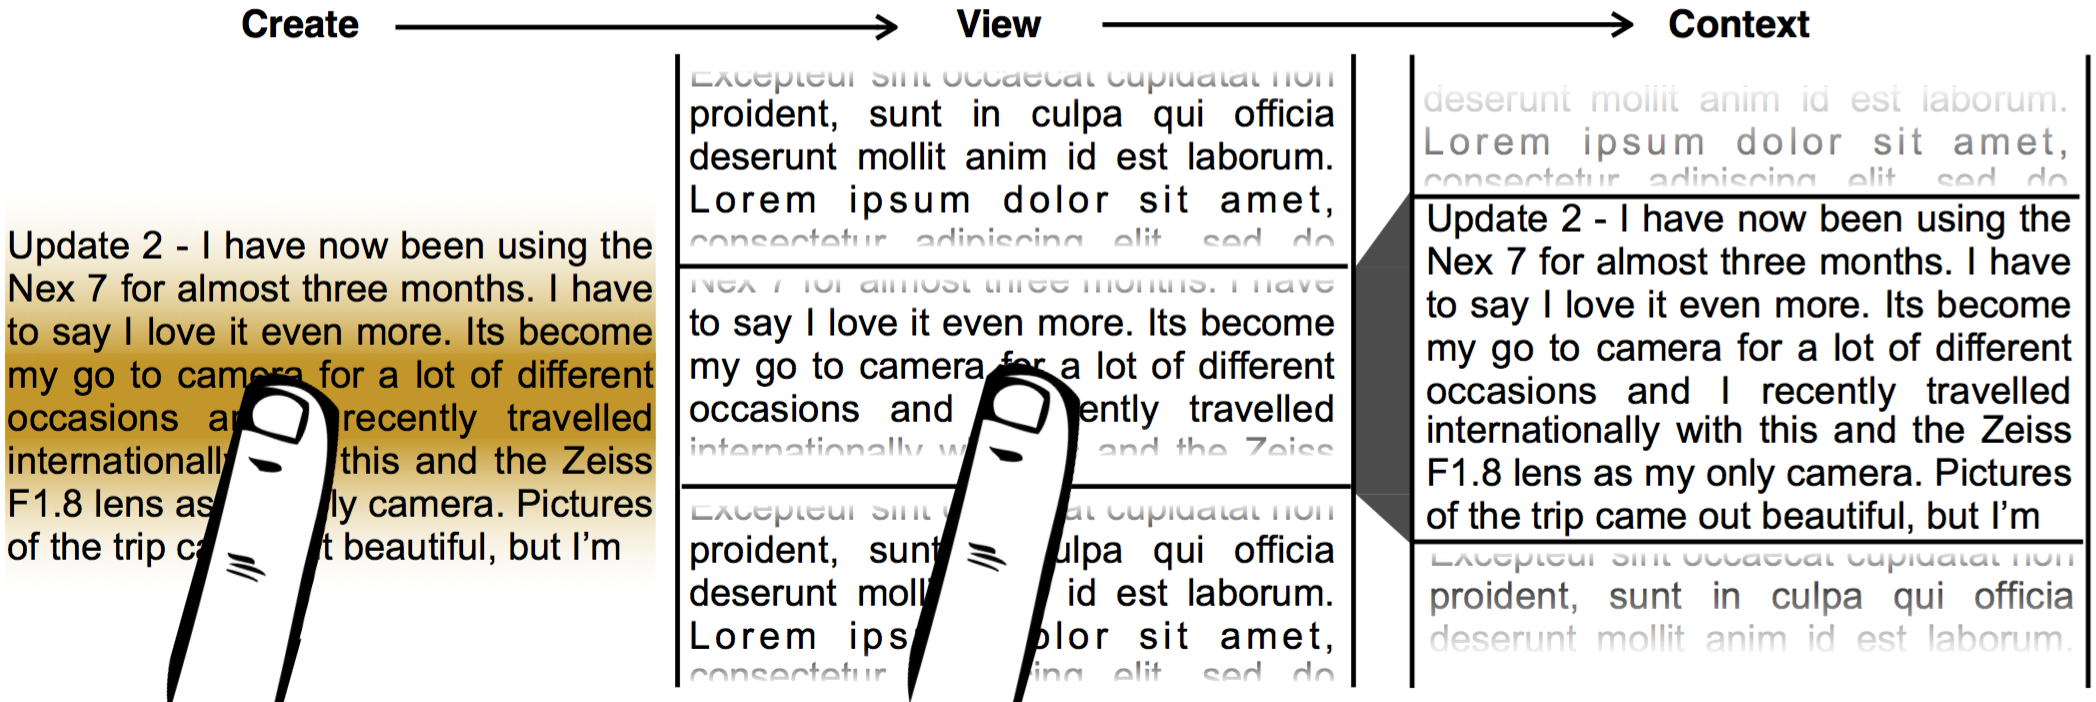
\includegraphics[width=0.8\columnwidth]{Chapters/Highlight/img/system.png}
    \caption[Fuzzy highlighting interaction and corresponding viewer]{Highlighting with intentionally fuzzy boundary and a viewer that supports resolving uncertainty.}
    \label{fig:fuzzy}
\end{figure}


\section{Introduction}

Capturing information online for later use can be especially challenging during exploratory search tasks \cite{Capra:2010:TLM:1753326.1753468}. Studies of information foraging \cite{pirolli1999information} and active reading \cite{morris2007reading} have identified the importance of collecting snippets of information while exploring and reading from multiple sources for comparison, cross-referencing, and structuring \cite{kirsh1995intelligent, adler1998diary, tashman2011active, kittur2013costs}. As reading and learning increasingly moves from handwritten notes and highlighted pages into web search and browsing, tools for supporting the curation and storage of online information have grown in popularity. For example, one well known tool for extracting snippets of information from web pages -- Evernote Web Clipper -- had over 4 million users on the Chrome desktop browser alone\footnote{http://chrome.google.com/webstore/}.

The need for reading and capturing information has expanded beyond the desk to domains where mobile devices are prevalent, such as in bed or at the kitchen table \cite{ adler1998diary,tashman2011active}. Despite this need, identifying and saving snippets of textual information remains challenging on mobile devices. Small screens and font sizes combined with the inaccuracy of touch interfaces make selecting and saving text both time consuming and stressful. To understand the prevalence of text highlighting scenarios on mobile devices today, we conducted a survey with 153 participants (age 20-59, mean 32, 60\% male, 76.5\% from the U.S.) asking for their experiences with complex exploratory searches \cite{marchionini2006exploratory} on smartphones. Our results suggest that people frequently conduct complex searches either partly (70\%) or completely (45\%) on their phones. When asked about what makes these searches difficult, near half agreed that ``\emph{Selecting part of a webpage and save it}'' is either moderately or extremely difficult, and 41\% thought it would be valuable to have a better interface for it.

Approaches to improving capture interfaces have, to date, focused on improving the speed and accuracy of specifying the start and end boundaries of the selection area. Such approaches include using bezel or multi-push gestures \cite{chen2014bezelcopy, roth2009bezel, han2015push}, autocomplete \cite{zhao2012autocompaste}, switching windows faster \cite{chapuis2007copy, faure2009power}, or leveraging the structure of the content to be copied \cite{bier2006entity, ives2009interactive, stylos2004citrine}. These approaches are well suited for fast and simple copy-paste needs, such as copying an address from one application and pasting it in another.



%However, developing a better interface for capturing information on mobile devices as people are reading also requires a deep consideration of the process that people engage in as they are learning or making sense of a new domain. 

%At the present, many smartphone information foraging support tools rely on the existing select-copy-paste metaphor native to devices. This is limiting, due to the hard boundaries imposed, and the lack of uncertain input inherent to exploration. For example, on iOS and Android devices a user initiates text selection mode by tapping and holding one finger on the screen for about 0.5 seconds and releasing their finger from the screen. Two draggable handles will then appear for specifying the start and end characters. Researchers have looked at how to speed this process up, 

%Because of the difficulties in using annotation tools in a digital medium, users often still prefer paper-based mediums for annotation \cite{tashman2011active}.
%\nathan{I changed this last sentence} 

%In these approaches, the user or system must specify hard boundaries for both ends of the selection area. 


However, in many learning and exploration tasks, people are uncertain about which and how much information to save. Early in the process, before a user has a good sense of the topic space, they might save information that later turns out to be irrelevant, or they may be uncertain about how much information on a particular page may be needed in the future \cite{kittur2013costs}. For example, a researcher might extract a particular finding from a paper early in their exploration process, only to realize later that they also need the author's statistical model from the following paragraph. Conversely, over-selecting text that does not prove to be useful later can lead to additional effort in sifting out useful information from extraneous chaff (for example, in the limit if the entire page was selected and saved then the user would have to do all the filtering again). Furthermore, forcing a user to choose hard selection boundaries requires them to carefully predict their future information need, which can involve high cognitive effort \cite{sinha2005cognitive}. Indeed, in a pilot survey, we found 11 out of 19 participants had trouble in the past identifying how much text to highlight. Additionally, 13 out of 19 mentioned that they had needed to return to a document to read additional text in order to understand the selections they created in the past. These findings suggest that these considerations are commonly encountered. Adding to the challenge, interactions for gathering information while reading need to be quick and low effort, otherwise people tend not to capture information in the first place \cite{marshall2005saving,tashman2011liquidtext,hinckley2012informal}. 

%determining how much information to save early in the process is often difficult, making fixed, context-less highlights impractical. For example, a researcher might extract a particular finding from a paper early in their exploration process, only to realize later that they also need the author's statistical model from the following paragraph. Early in the process, before a user has a good sense of the topic space, they might save information that later turns out to be irrelevant, or they may be uncertain about how much information on a particular page may be needed in the future \cite{kittur2013costs}. 

%Even more so, selection and highlighting on current mobile devices impose hard boundaries and high costs for incorrect selections. 

%which may be difficult to do if they are uncertain of the value and/or the extent of information they will need later.
%Beyond the challenge of simply selecting a region of bounded text on a mobile device, 


In this chapter, we introduce and explore the concept of intentionally supporting uncertain input in the context of selecting and saving information during information exploration on mobile devices. We investigate the idea that in contrast to more defined selection tasks (such as copying an address or phone number), precise selection may not be the most appropriate interaction paradigm for complex learning and reading tasks. In doing so we build on previous approaches that support fuzzy input, encourage lower granularity selection (e.g., lines of text vs. characters), or defer action until later \cite{schilit1998beyond,lank2005sloppy, tashman2011liquidtext,hinckley2012informal,kittur2013costs,schwarz2015architecture}
In contrast to approaches which take uncertain input and maintain its uncertainty to be resolved later (e.g., \cite{schwarz2015architecture}) in which the user intention is certain but the input is not, we suggest that there are cases in which the user intention is itself uncertain and resolving user input is inappropriate. This approach frees us to consider alternate ways to support selecting and saving information, especially on mobile devices where selecting and saving can be challenging for users. 

Specifically, we explore two ways in which we can design for intentionally uncertain input. One is to support uncertainty in the selection interface through a fuzzy bounding box. This allows a user to feel less stressed about exactly where the boundaries of their selection lie and may reduce the need for careful prediction of their future information need. Another way is to support uncertainty in retrieval by saving context around the selection area and surfacing it later. We explore the tradeoffs of these two approaches and their interaction through a controlled experimental study.
Furthermore, we introduce the idea of using pressure-sensitive touch as a new interaction approach for specifying selection boundaries. Pressure is particularly interesting as a modality because it has the potential to allow the fast selection of an area of interest while relaxing the cognitive and physical constraints of needing to specify exactly what should be saved. One potential drawback of such an approach is missing the information needed later due to inexact boundary selection, which motivated the idea of expandable context when reviewing snippets later. 
%we argue that an important user interface consideration in the learning and exploration process is designing for intentional uncertainty in the process. This uncertainty is fundamental to supporting the process of trying to identify important information that should be saved, and trying to estimate the correct context to both minimize the likelihood of missing something and reducing the amount of information that needs to be reread and filtered when using the information in the future. 
%In a larger scope, researchers have also been developing interactive systems to better support active reading and exploratory search on digital devices \cite{schilit1998beyond, tashman2011liquidtext,hinckley2012informal,kittur2013costs}. 
%In particular, Hinckley, et. al described two patterns for lowering the transaction cost of saving information while reading. First, deferring part of the actions to a later time. For example, separating and deferring annotation and categorization actions from when highlights are saved. 
%It may seem that splitting and deferring interactions could create additional cognitive cost due to lost of context, but Kittur, et al. have shown that in early stages of exploration, users often do not have enough knowledge to label gathered information effectively, and deferring parts of an interaction to a later time can actually be beneficial \cite{kittur2013costs}.
%Second, relaxing the precision of the interaction \cite{pohl2013focused}. For example, only allow users to highlight blocks of text instead of specifying character ranges \cite{hinckley2012informal}. Notice past systems have explored limiting the granularity of text selection (i.e., lines instead of characters), the input boundaries are still certain to the users at all times
%(i.e., first character of a line and last character of another), whereas in this paper, we explore the concept of uncertain input by intentionally hiding the precise boundaries from the users.
In the rest of the chapter, we will first describe the specific design of a system that embodies intentionally uncertain input in both selection (through pressure-sensitive touch selection) and retrieval of information. We then describe a two-part user study in which we investigate the performance of the two types of interfaces for a low-uncertainty task (targeted copy-paste) and a high-uncertainty task (exploratory search). 



% In two studies we found that the proposed approach is preferred over the iOS default text selection function by 19 out of 19 participants, significantly (TODO analysis) reduced user workload on interaction time and stress level during a complex sensemaking task commonly to exploratory searches. 



% \section{Related Work}

% Text selection: push-push (UIST’15), BezelSwipe (CHI’09), BezelCopy (AVI’14)

% Highlighting: ?

% Context: ?

% Uncertain input. E.g., Julia Schwarz’s work and others on touch input and interface uncertainty

% Comparing to system and many other previous approaches (push-push/bezel copy), the entire operation is done in single touch session (only one release), and potentially more time efficient. The trade off: max size / sub-line accuracy, discuss more in limitation and future work.)

\section{System Design}
In this section, we introduce a new highlighting interaction that supports intentionally uncertain selection. Our aim with this technique is to reduce the stress and increase the efficiency of saving information for future use while exploring and learning new information. The explain this interaction, we break up the process of highlighting into three separate steps: initiating selection mode, indicating the start and end points, and saving the selected text. In the remainder of this section, we will give a high level overview of the proposed highlight interaction, and then discuss the different design options we explored for each step in the interaction.

\begin{figure}
    \centering
    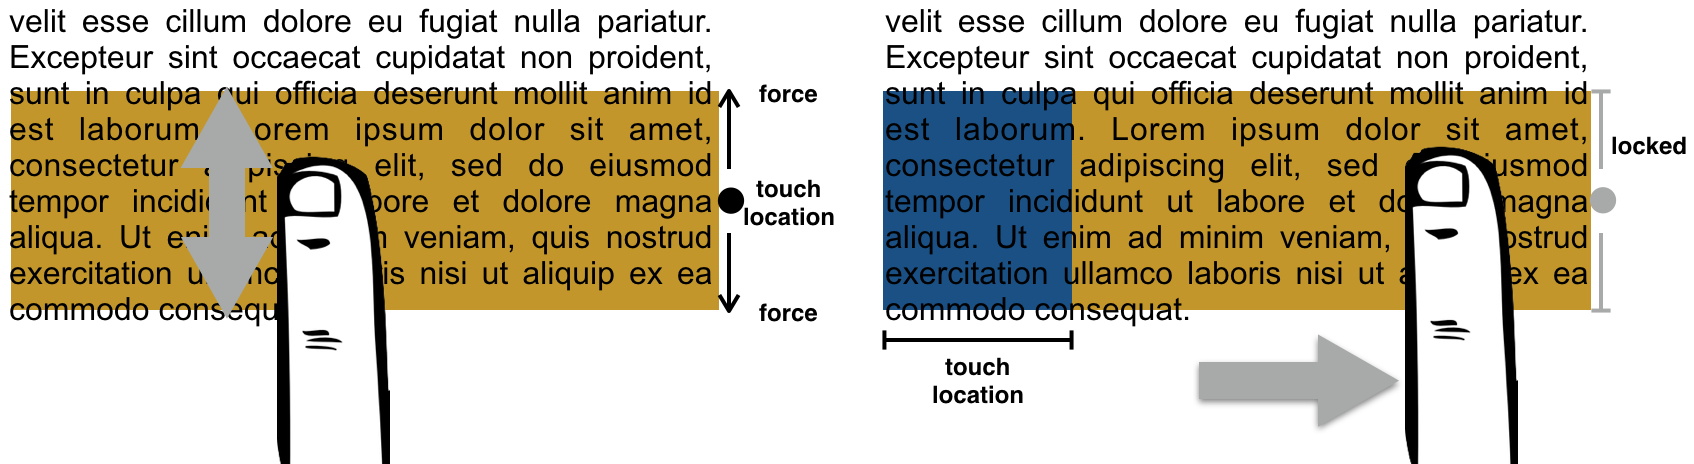
\includegraphics[width=0.8\columnwidth]{Chapters/Highlight/img/system2}
    \caption[Proposed interaction for selecting and saving text on force sensitive touch screens.]{Selecting and saving text using force to set the selection area (left) then sliding right to lock it.}
    \label{fig:system}
\end{figure}


\subsection{Selection Interface}

The proposed interaction is composed of three steps, which align with the above mentioned process (Figure \ref{fig:system}): 
\begin{enumerate}
    \item Users initiate selection mode with a pressure (force) touch on the general area of interest. 
    \item Once selection mode is enabled, they then estimate the amount of context needed in the future by controlling their force while moving their fingers vertically to fine-tune the start and end points. 
    \item Finally, they swipe horizontally to confirm and save the information.
\end{enumerate}

We explored three options for initiating text selection mode. One way is to use a simple touch gesture to start text selection, and swipe your finger across select text. This is analogous to using a highlighter pen to highlight text on papers. However, on a smartphone this may conflict with a number of gestures in reading mode, such as scrolling or canceling a tap on a hyperlink. The second option is to use the time dimension to initiate text selection to avoid conflicts with the reading mode gestures, such as tapping and holding at the same location for 500 milliseconds on iOS and Android devices. However, this will add an inherent cost to every highlight the user creates. 500 milliseconds might seem like a low cost if text selection is rarely needed. However, when people engage in complex sensemaking tasks, such as exploratory search, they often have the need to save pieces of information frequently in a short period of time \cite{teevan2006personal}. The third option is to use the force dimension, which is beginning to appear in mass market products, to trigger text selection. This has the benefits of having no conflict with existing reading mode gestures and virtually no time delay. Consequently, we choose the third option for initiating our text selection phase.

In designing the interaction for the selection mode, we explored four options for indicating the start and the end points. The first option is to use two draggable handles for indicating the start and the end positions, and the second option is to use the initial touch location as the start point and the release location as the end point. Both approaches are used by many current touch systems, but both suffer from the inaccuracy of finger based touchscreens (minimal target area of 44 by 44 pixels) and the small font size (default of 17 points, or 34 pixels on iOS), making it difficult to physically pin-point the intended characters. Further, the finger view-blocking problem makes it difficult to for user to do fine-grained adjustments. To avoid having the users tap on exact words or characters, we instead chose the third option, which takes the touch coordinates as the center of the selection and uses the amount of force to determine the size of the selection. We explored two sub-options for adjusting selection range based on the amount of force. We first tested using force to adjust selection range at the character or word level. However, it was difficult to keep track of the start and the end points at the same time, especially near the beginning and the end of each line. The second option is to use force to adjust how many lines are selected. This way, the start and the end boundaries have the same vertical distance to the touch location, and was much easier to keep track of at the same time when adjusting the amount of force used. We tested mapping the same amount of force used to the same number of pixel height and number of lines highlighted according to the font size of the page. The second option made the system more consistent on pages with different font sizes, and also aligns better with our design goal of correlating force with the amount of context required by the user.

Finally, for saving the selection, we explored two options. The first is to have users quickly release their fingers from the touchscreen to save the selected text. Our pilot studies showed this option to be intuitive, and often what the users try first. However, in practice this approach proved challenging as it made capturing the right selection range ambiguous, since the force dimension is also used to control the range of the selection. Similarly, in our lab study some participants encountered similar issues with the built-in text selection, and often accidentally moved the handles when releasing their fingers from the screen. Instead, in our approach users move their finger horizontally across the screen and then release to save the selected text. By using a new dimension, we reduce the chance of accidentally changing the selected range when leaving the selection mode. To reduce the number of dimensions the users need to control, we lock the selection range (both the center location and the size) once the user begins to swipe their finger horizontally. 

Previous work has shown conducting gestures in the force touched state can be laborious \cite{Lee:2014:DIT:2686612.2686702}. However, in our design, we only make use of the Y dimension movements during the selection mode, and we lock both the Y dimension and the  force dimension when the user starts moving their fingers horizontally in the saving mode (Figure \ref{fig:system}). User studies showed that participants were both able to efficiently create highlights using the proposed mechanisms, and prefer using the proposed interaction over the built-in text selection feature with draggable handles for highlighting information during a complex sensemaking task.
 

\begin{figure}[ht]
    \centering
    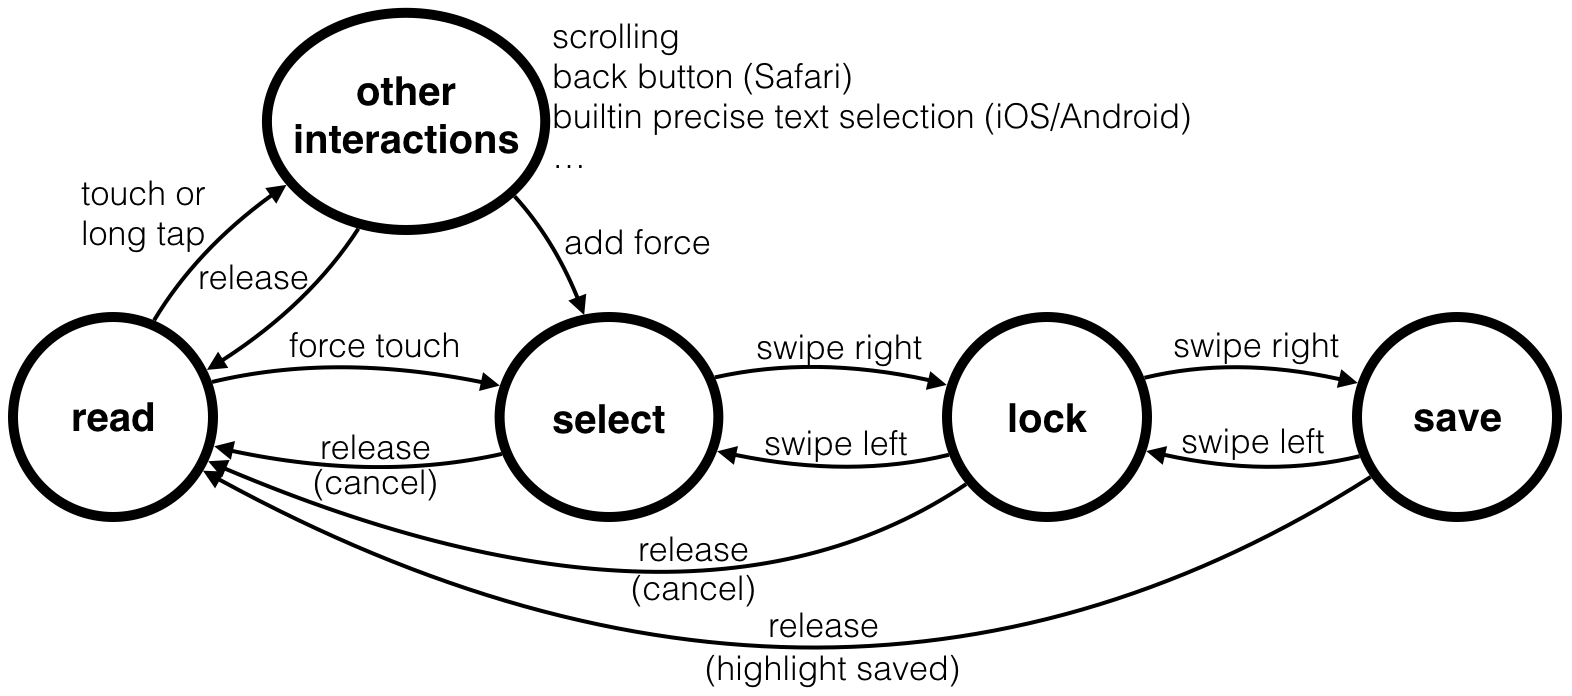
\includegraphics[width=0.8\columnwidth]{Chapters/Highlight/img/states.png}
    \caption[State transition diagram for the uncertain highlighting interaction technique.]{State transition diagram.}
    \label{fig:states}
\end{figure}

%\begin{table}
%    \centering
%\begin{tabular}{ l l l l }
%\hline
%Phase & X coordinate & Y coordinate & Force \\ 
%\hline
%Selection  &(not used) & selection center & selection %size\\
%Saving  & lock \& save & (not used) & (not used) \\
%\hline
%\end{tabular}
%    \caption{Dimensions used at different stages of %the operation.}
%    \label{tab:dimensions}
%\end{table}


Figure \ref{fig:states} shows the states and transitions of the proposed interaction. Notice that the proposed interaction does not interfere with common reading interactions, such as vertical scrolling or horizontal swiping (backwards and forwards buttons in Safari). In addition, the proposed interaction can also co-exist with common precise text selection methods (both commercial and academic) that are initiated with long taps or edge taps \cite{chen2014bezelcopy}. We will discuss about supporting multiple selection methods in the discussion section.

\subsection{Intentionally Uncertain Boundary}
%Admittedly, with the highlighting operation design described above, users will not be able to adjust highlight range at the character or even word level as they would using the built-in text selection features on Android or iOS. However, our pilot survey suggests that forcing people to select exact ranges for highlighting during the exploratory search process may be a source of stress, as the users can be uncertain about the amount of context needed to understand the information in the future, especially early in the process. This hints that uncertainty might be a key design consideration for highlighting new information, and lead us to believe that designing a new interaction with intentionally uncertain input at the time of saving have the potential of greatly reduce the stress and the effort involved in highlight important information during exploratory search or other sensemaking tasks involving learning new knowledge.

%\begin{figure}
%    \centering
%    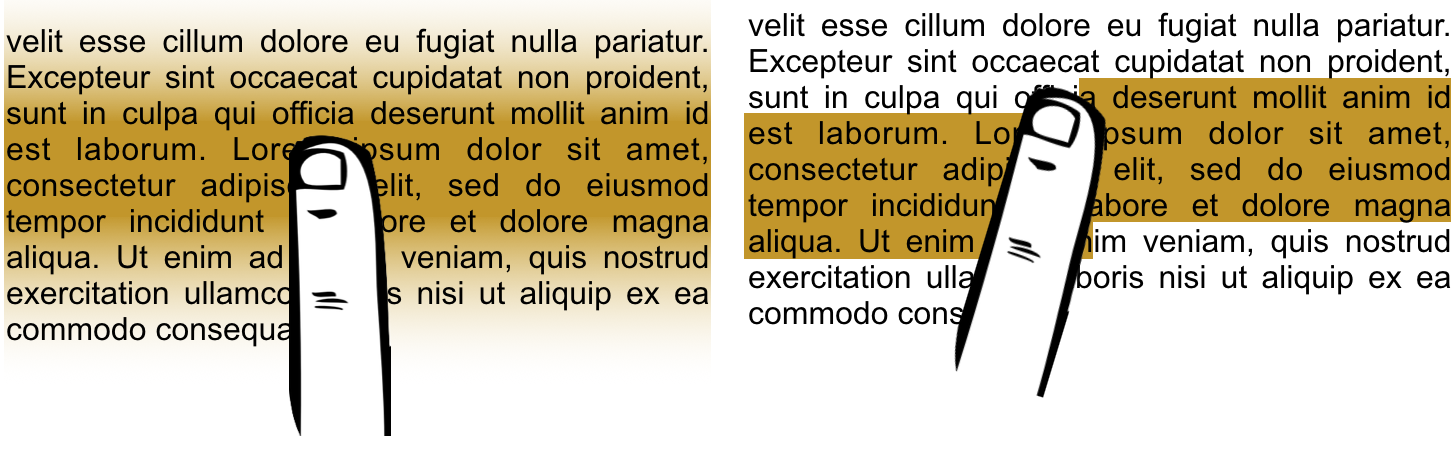
\includegraphics[width=8cm]{img/fuzzy_front.png}
%    \caption{Highlighting with intentionally fuzzy boundary and precise character boundary.}
%    \label{fig:fuzzy}
%\end{figure}

We explored designing for uncertainty in two complementary ways: through a fuzzy boundary during highlighting, and through an expandable context during review. To explore uncertain input as a design consideration for highlighting, we introduced a fuzzy boundary in the selection mode (Figure \ref{fig:fuzzy}). By intentionally hiding the hard boundaries from the user, we hope to free them from engaging in the difficult task of determining exactly how much context they will need when creating highlights, and postpone uncertainty resolution until the users review the saved information with a better idea of how much context they need. To achieve this, whenever the user creates a new highlight, the system will also save its surrounding text as context. To give users dynamic access to the context when reviewing, we made a simple highlight list interface that allows the users to use force touch gesture to expand the viewport and request for more context. The idea is that knowing they will have the chance to adjust the amount of context for each highlight during the review process, it will reduce both the cognitive stress and physical interaction load of creating highlights with exact boundaries.

%\begin{figure}
%    \centering
%    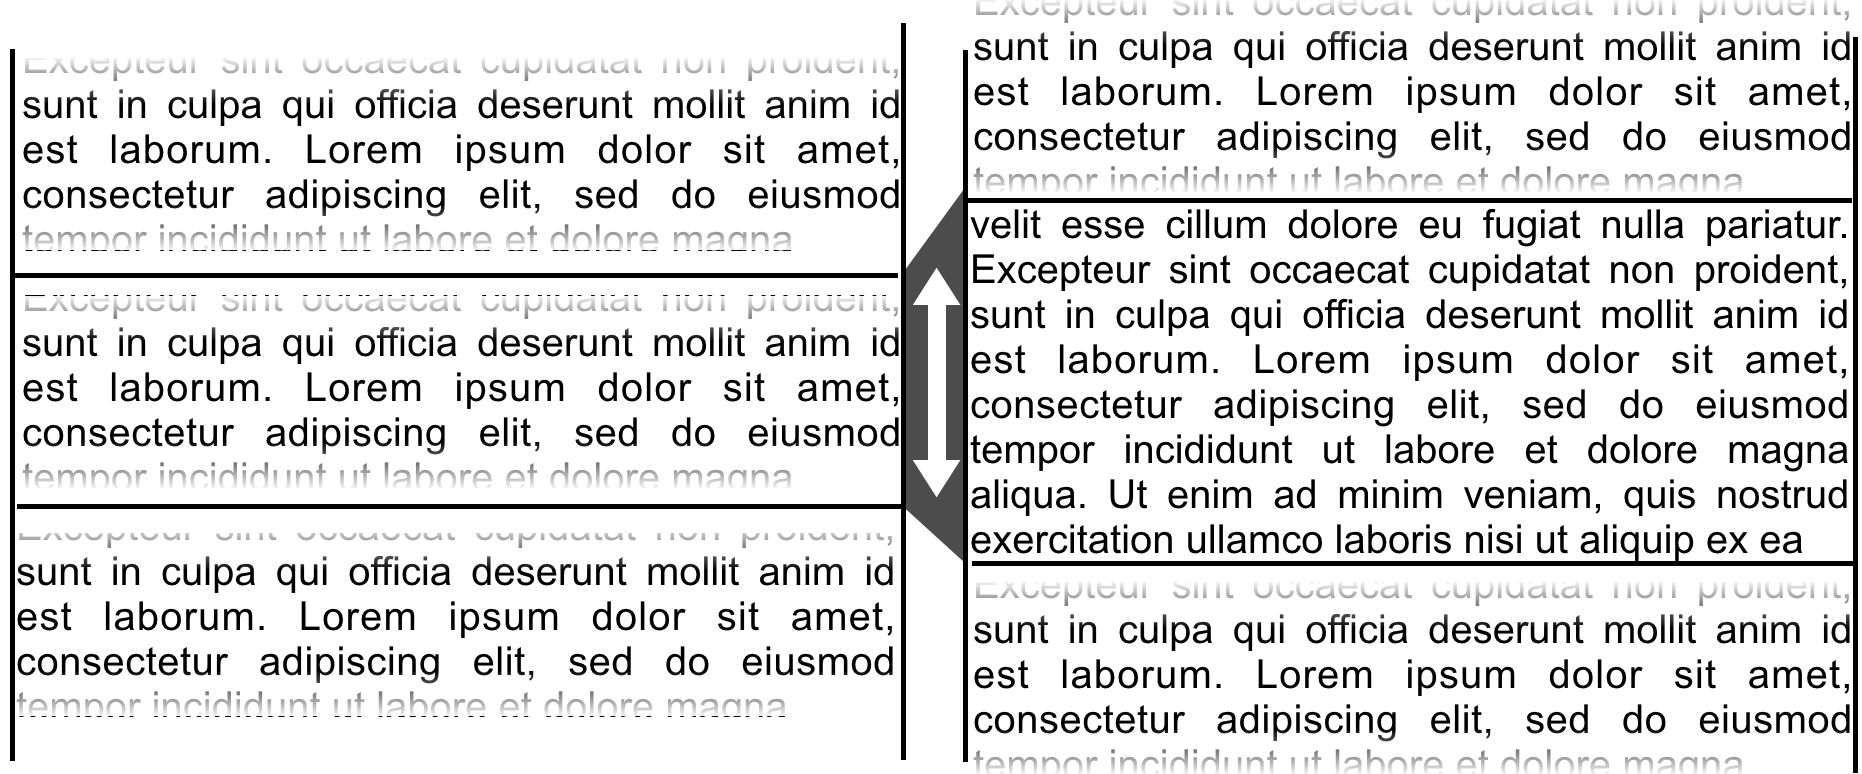
\includegraphics[width=8cm]{img/viewer.png}
%    \caption{Highlight viewer that supports resolving uncertainty.}
%    \label{fig:viewer}
%\end{figure}

%In our user study, we use input uncertainty as a within-subject variable with three highlighting modes, and use the ability to resolve uncertainty when reviewing as a between-subject variable. With this study design, we can compare the users’ preferences and stress level using certain and uncertain input, as well as how having the ability to resolve uncertainty later affects their opinions about the input methods.

\begin{table}
    \footnotesize
    \centering

    \begin{tabular}{l r r r | r r r | r r r }
    
     & \multicolumn{3}{c|}{\textbf{Study 1}}
     & \multicolumn{3}{c|}{\textbf{Study 2 (with context)}}
     & \multicolumn{3}{c}{\textbf{Study 2 (no context)}} \\
    
     & Hard & Fuzzy & System
     & Hard & Fuzzy & System
     & Hard & Fuzzy & System \\
    \hline
    Mental 
    & 7.43 & 6.10 & 9.05
    & 6.78 & 5.89 & 8.33
    & 7.50 & 5.90 & 10.50 \\
    Physical
    & 7.57 & 6.00 & 9.05
    & 8.11 & 5.56 & 10.22
    & 6.10 & 3.90 & 9.20 \\
    Temporal
    & 7.90 & 7.10 & 9.52
    & 8.22 & 6.56 & 11.00
    & 6.50 & 6.60 & 9.80 \\
    Performance
    & 14.10 & 15.00 & 13.43
    & 12.44 & 14.00 & 12.11
    & 12.20 & 15.30 & 14.30 \\
    Effort
    & 8.86 & 6.76 & 11.00
    & 7.78 & 5.00 & 9.33
    & 6.20 & 6.10 & 10.80 \\
    Frustration
    & 7.43 & 5.19  & 11.52
    & 7.00 & 4.00 & 11.00
    & 5.10 & 4.80 & 8.90 \\
    \hline
    \textbf{Overall (0-100)}
    & 39.20 &31.10 & 50.14
    & 37.89 & 27.00 & 49.89
    & 31.40 & 27.30 & 49.20 \\
    
    
    & & & N=24
    & & & N=9
    & & & N=10 \\
    \end{tabular}
    
    \caption[NASA TLX scores for three highlighting modes.]{Average NASA TLX scores for three highlighting modes from part 1 of the lab study: Targeted highlighting (left), reading and highlighting with an expandable viewer (middle), and without an expandable viewer (right). Higher numbers mean higher workload or higher performance.}
    \label{tab:nasa_train}
\end{table}



\section{User Study}
We conducted a two-part lab study to evaluate three highlighting methods for saving information during exploratory search for later use: force touch with hard boundary, force touch with fuzzy boundary, and system selection. The first part of the study tested the overall interaction workload without the cognitive demands of exploratory search, while the second part added simulated exploratory search behaviors. In the first part, individuals were given articles and asked to highlight random portions selected by the system for 20 minutes. In addition to collecting data, this served to train participants to use the three modes efficiently. In the second part of the study, participants were given a complex sensemaking task involving reading multiple articles and creating their own highlights. Afterwards, they reviewed their highlights using either an interface which showed expanded context around their initial selection or that only included their original selection, and wrote a short summary integrating the content of the articles. 

We implemented the proposed technique on an iPhone 6s Plus running iOS 9.3.3 through a custom native app that uses the standard WebKit browser for the reader interface. Force touch highlighting was implemented in Javascript by accessing pressure sensor data through WebKit APIs and injected into the WebKit reader using Cocoa APIs.


\subsection{Demographic}

We recruited 24 participants from a local behavioral research participant pool. Participants ranged in age from 18 to 59. The majority of the participants were either undergraduate or graduate students, 11 female and 13 male. Participants were required to be fluent in English and use a smartphone as their main mobile phone. Based on self-reporting, 14 were Android users and 10 iPhone users. 


\subsection{Lab Study Part 1: Training and Interaction Cost}

In the first part of the study, we evaluated the interaction cost of three highlighting methods: force touch with hard boundary, force touch with fuzzy boundary, and system selection. To remove the effects of prior knowledge and the cognitive demands associated with learning new information, the system marked random portions of article in red and asked participants to only highlight the red sentences without actually reading the article. Participants were required to highlight the sentences completely without highlighting surrounding sentences in order to proceed.

\begin{figure}
    \centering
    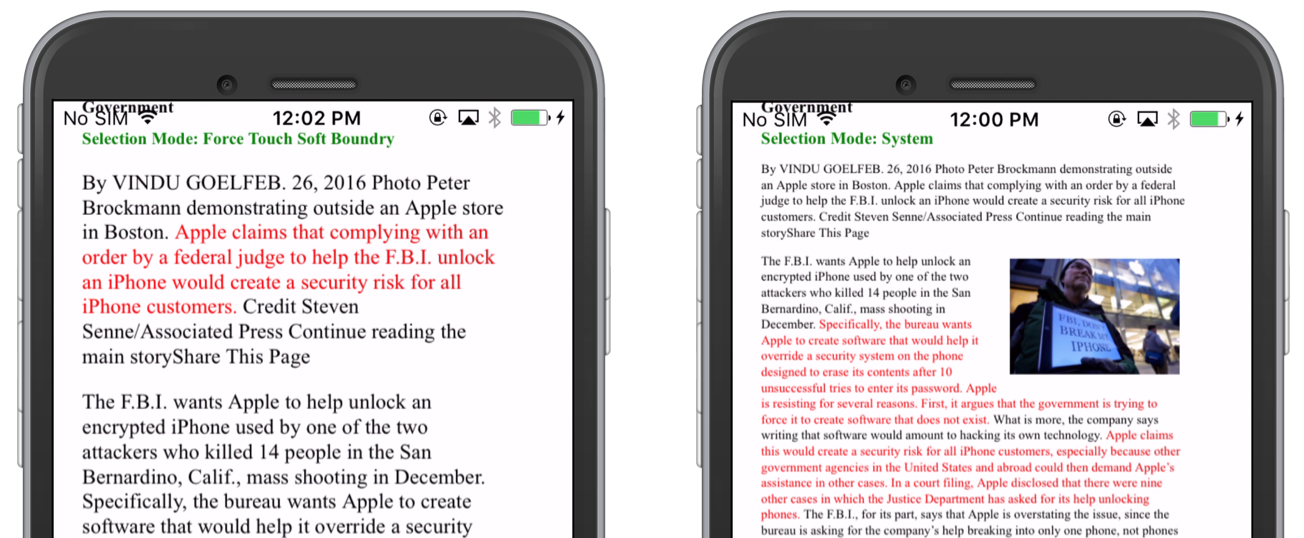
\includegraphics[width=0.8\columnwidth]{Chapters/Highlight/img/training.png}
    \caption[Examples from the lab study]{Examples from Part 1 of the lab study, where participants were asked to create highlights covering the red lines. Pages varied in conditions including font size and page layout.}
    \label{fig:training_screenshot}
\end{figure}

Before the study began, individuals filled out a pre-survey for demographic information and how they currently used text selection or highlighting on their smartphones. During the study, participants were given a minimum of 24 pages (8 for each mode) in random order. On each page there were four highlight targets (32 for each mode). We also randomized the font sizes (30px, 38px, 47px), page layout (with/without photos), and location and size of the targets (3-8 lines).  If they finished highlighting the 24 pages under twenty minutes, more pages with random conditions were provided. Afterwards, participants filled out a NASA TLX survey for each highlight mode \cite{hart1988development} to measure cognitive load.

\subsubsection{Results}

\begin{table}
    \centering
    \footnotesize
    \begin{tabular}{r | l}
    \hline
    \textbf{Question} & \textbf{Mean[.95CI]} \\
    \hline
I find it frustrating to select text on my smartphone & 5.71[5.19, 6.23]* \\
I find it time consuming to select text on my smartphone & 5.50[4.84, 6.16]* \\
I can select text efficiently on my smartphone & 3.17[2.50, 3.83] \\
I often copy and paste text on my smartphone & 3.92[3.09, 4.74]* \\
I often highlight text on my smartphone & 3.17[2.50, 3.83] \\
I would copy or highlight text more often if it was easier to do on my smartphone & 5.79[5.26, 6.32]* \\
    \hline
    \end{tabular}
    \caption[Self-reported text selection and highlighting habits.]{Self-reported text selection and highlighting habits on a 7-point likert scale. A higher score indicates stronger agreement. N=24}
    \label{tab:text_selection}
\end{table}


Table \ref{tab:text_selection} shows the pre-survey responses from 24 participants about their smartphone text selection habits and opinions. The results show that many users find it frustrating and time consuming to use the text selection feature, and they are unable to do it efficiently or frequently. However, 22 out of the 24 participants agree that they would copy or highlight text more often if it was easier to do so. This suggests a strong need for saving information for future use on smartphone devices, and the lack of an efficient method to fulfill this need. 

When asked about the reasons for copying and pasting on their smartphones, 63\% of the participants reported copying text for later use with note taking apps or emailing themselves, and 58\% reported copying text to share information with friends via social networks, emails, or text messages. For none textual copying and pasting, 54\% of the participants reported sharing URLs with friends, and 50\% reported saving URLs for themselves. Finally, 21\% of the participants reported to not use the copy and paste feature. 


\begin{figure}
    \centering
    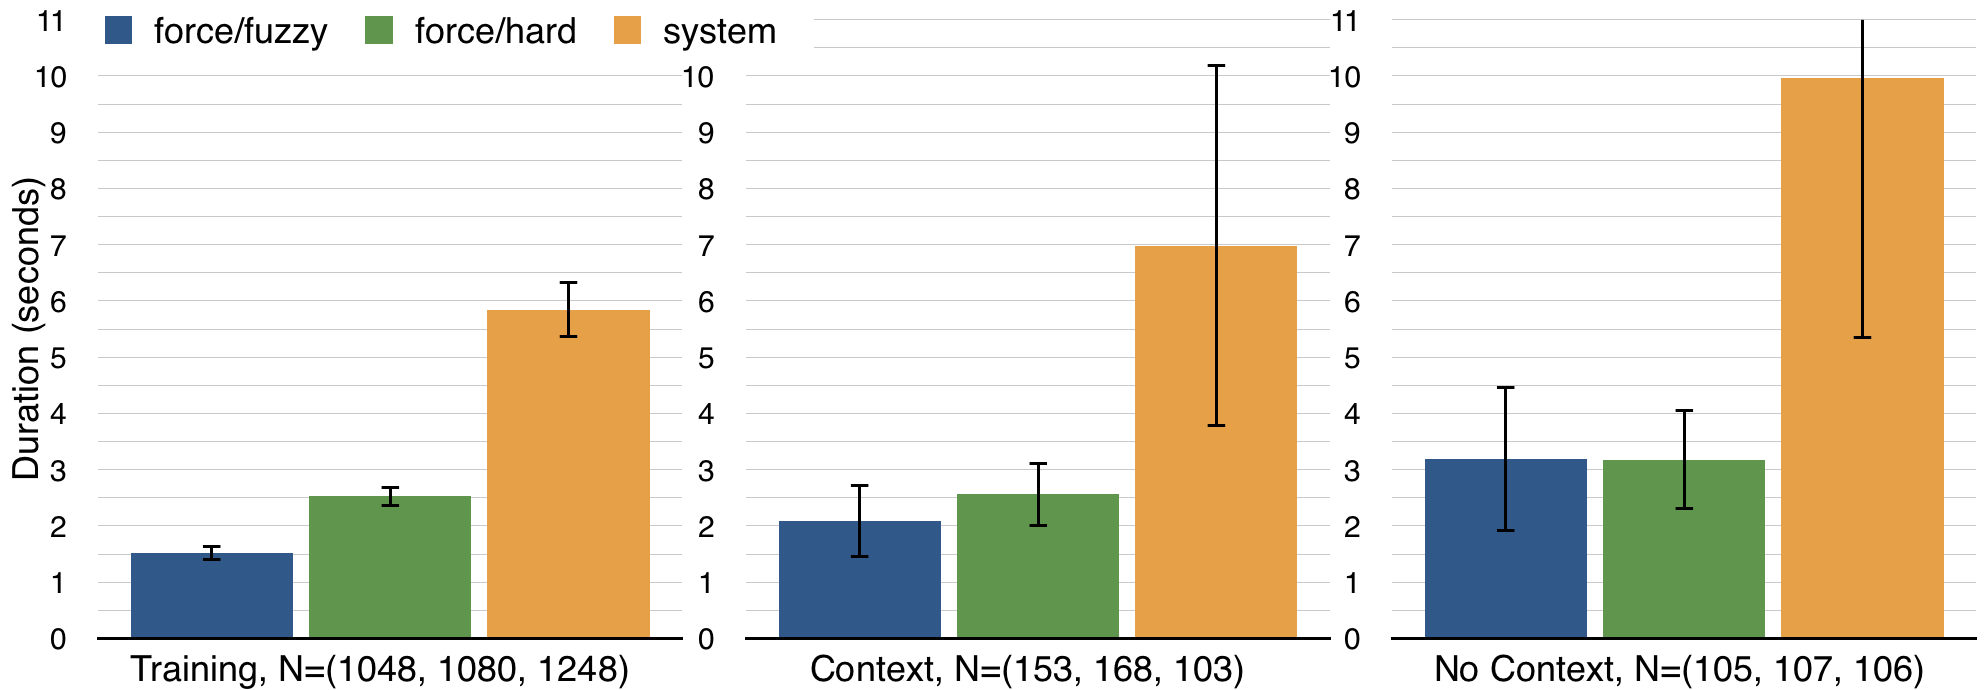
\includegraphics[width=\columnwidth]{Chapters/Highlight/img/runtime.png}
    \caption[Average time spent creating highlights under different conditions.]{Average time spent creating highlights in each condition: training in part 1 (left), the context condition in part 2 of the study (middle), and the no context condition in part 3 of the study (right)}
    \label{fig:highlight_runtime}
\end{figure}

Based on 1048 samples for force highlight with fuzzy boundary, 1080 samples for force highlight with hard boundary, and 1248 samples for system selection, the average time to create highlights using the three modes were 1.80 seconds, 2.77 seconds, and 6.06 seconds, respectively (Figure \ref{fig:highlight_runtime}). We analyzed these results using an ANOVA model, where duration was found to be significant different between the three conditions (F(2,20) = 18.0, p \textless  0.001). Using a Fisher LSD means difference test, we found the soft boundary selection mode was the fastest, with the hard boundary mode being slightly slower, and system selection being the slowest (p \textless 0.001). Note that these times reflect the constraint that users were not able to proceed without accurate highlighting. No significant differences were found on NASA TLX measures. In the next study, we look at how this new highlighting technique perform when users are actively engaged with the content through a complex sensemaking task. 


\subsection{Lab Study Part 2: Exploratory Information Seeking}

In the second part of the study, individuals were asked to highlight important information while researching a new topic, and to write a short summary using the highlights they created. Half of the participants were given the reviewing interface in which they could expanding context surrounding their original highlights. 

First, participants completed a pre-survey about their experiences and opinions about saving information for future use on mobile devices. Before they started on the main task, individuals were given six highlights we created from the Planet Habitability entry from Wikipedia and asked to write a short summary of the six highlights in five minutes. This was to ensure the participants in the context condition were aware that they could resolve uncertainty when reviewing their highlights when they wrote the summary. Finally for the main task, participants were given three pages to read, each containing two Amazon reviews for a different camera. Participants were told they had 15 minutes to read and highlight each source, and all three sources were of similar length, so they should spend roughly five minutes on each page. Each page required the participants to use a different method to create highlights; both the pages and modes were given in random order. After 15 minutes, participants were given 10 minutes to review their highlights, rank the three cameras, and explain their reasoning. The instructions were as follows: 

``You have a friend who is looking to buy a new camera for taking pictures of his/her young kids at birthday parties. Using the highlights you saved, rank the three cameras, and write a short summary to explain to your friend how and why you ranked them this way.''


After writing the summary, individuals answered a NASA TLX survey for each highlight mode according to when they were created their own highlights on the camera articles, as well as a questionnaire about the three highlighting modes and highlighting information in general.

\subsubsection{Results}

\begin{table}
    \centering
    \footnotesize
    \begin{tabular}{r | l}
    \hline
    \textbf{Question} & \textbf{Mean[.95CI]} \\
    \hline
Soft boundary makes it less stressful to create highlights than the other two modes & 5.89[5.25, 6.54]* \\
Hard boundary makes it less stressful to highlight comparing soft boundary & 3.00[2.25, 3.75] \\
The system selection mode is less stressful to create highlights & 2.05[1.51, 2.60]* \\
Its fun to use the force touch with hard boundary mode to create highlights & 3.58[2.77, 4.39] \\
Its fun to use the force touch with soft boundary mode to create highlights & 5.32[4.61, 6.02]*  \\
    \hline
    \end{tabular}
    \caption[Survey question about certain and uncertain boundary.]{Survey question about certain and uncertain boundary using a 7-point likert scale. A higher score indicates stronger agreement. N=19}
    \label{tab:fuzzy_survey}
\end{table}

A total of 19 individuals participated in the part 2 of the study, where 10 of them were given the highlight review interface with that supports expanding viewport for more context, and 9 of them were given a highlight review interface with static viewports. All of the 19 individuals also participated in part 1 of the study, and had twenty minutes training of the three highlighting modes.
Using a 7-point likert scale, user reported strong preference over having a uncertain input for highlighting during the complex sensemaking task of ranking digital cameras. On average, participants agrees (5.89/7.00) that the force mode with fuzzy boundary makes it less stressful comparing to force mode with hard boundary and the system selection mode, and find (5.32/7.00) using the force touch with fuzzy boundary mode to be fun (Table \ref{tab:fuzzy_survey}). When asked about which of the three highlighting mode they would use in the future if they need to read articles and learn new things on their phone, 15 of the 19 participants chose force touch with fuzzy boundary, 4 chose force touch with hard boundary, and 0 chose the system selection feature. In both conditions, only two participants chose the force highlighting mode with hard boundary, suggesting that even without the a way to resolve uncertainty when reviewing the saved information, some participants still prefer uncertain input while selecting and saving information. Below are  representative quotes from participants about the soft boundary force touch interface:

``The soft boundary took a bit of getting used to, but once I got the hang of it it made things go a lot faster. It took away the pressure of getting the exact lines right, and let my intuition take over about how much needed to be highlighted ''

``The soft boundary is my favorite, because it is the least physically taxing, least mentally taxing and if I'm going to highlight in an article it just has to be generally around what I want not perfect, so this was my favorite.''

``I hated how exact you had to be with the hard boundary.  It was just a huge pain. The soft boundary is so much better. I never realized how much I hated the generic copy and paste mechanisms. ''

We also asked the participants to fill out a NASA TLX survey for each of the three modes after writing the summary. To understand the workload effects, we utilized a generalized linear model to evaluate the differences between context vs no context, and the different modes of highlighting.  In the results of the model, context was not found to be a significant factor (F(1, 17) = 0.07, p = 0.789), however the highlighting mode was (F(2, 17) = 11.25, p \textless 0.01). Additionally, was no interaction effect between the level of context provided and the highlighting condition (F(2, 17) = 0.29, p = 0.749). In order to understand the difference between the three highlighting modes, we ran a Fisher LSD means difference test, and found both the force touch soft (t(17) = 4.66, p \textless 0.01) and the force touch hard (t(17) = 3.10, p \textless 0.01) conditions to be significantly easier at p \textless 0.01 than the system selection feature. There was no difference (t(17) = -1.56, p = 0.128) between the two force touch highlighting conditions. 

% However, the results did not show significant differences between the two highlight review conditions. 

%\begin{figure}
%    \centering
%    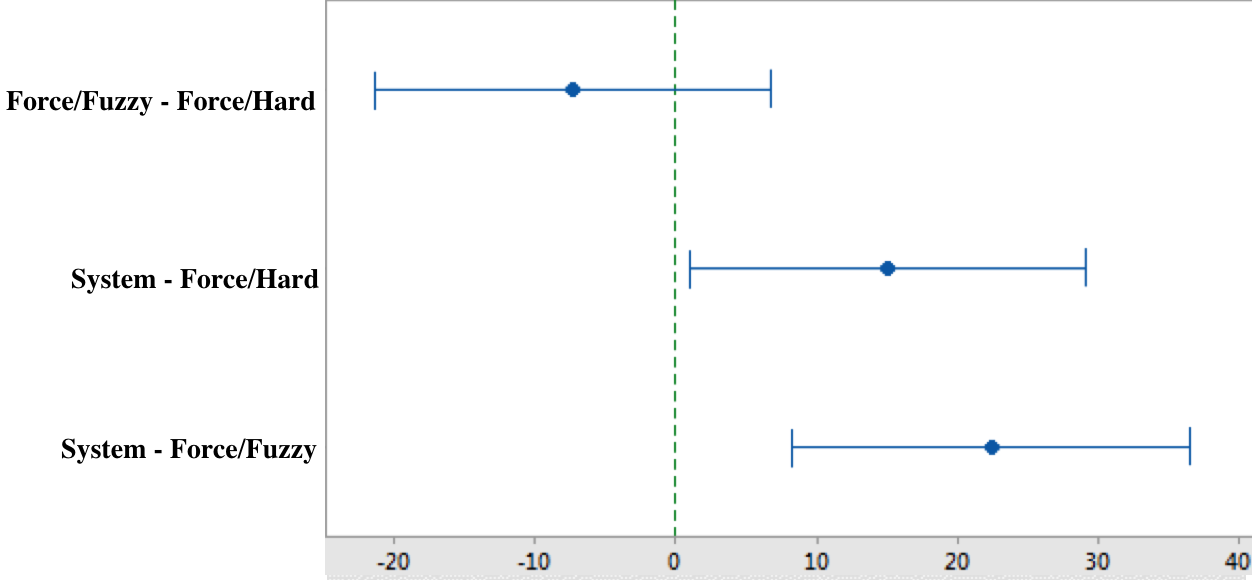
\includegraphics[width=8cm]{img/overall_p2.png}
%    \caption{Comparison of the NASA TLX overall score between %three highlighting modes based on all participants in part 2 of %the study.}
%    \label{fig:tlx_p2}
%\end{figure}
%

\section{Discussion}


We investigated the idea of interfaces that support intentionally uncertain input in the context of complex reading and sensemaking tasks, where precise input may be undesirable because it mismatches the high level of uncertainty in users' understanding of the topic space, leading to stress and poorer selections. To do so we developed a system in which users could highlight information on a mobile phone using force touch, and manipulated whether the boundary was hard or soft.  We also manipulated whether when they reviewed their highlights they could query for additional context around their highlights. Through a two-part user study we discovered that participants strongly preferred the force touch interaction technique with the soft, fuzzy boundary over the hard line boundary and over the default system selection with hard character boundary. We also found that both force touch highlighting approaches resulted in significantly faster selection speeds than the default system text selection.

%\nathan{I rewrote parts of this, make sure you like it} Overall, the user study was able to show the benefit of supporting intentionally uncertain input in situations where precision is actually undesirable and cumbersome. In the two-part study, we discovered that participants strongly preferred the force touch interaction techniques over the default system selection with hard character boundary. Additionally, we found that both force touch highlighting approaches resulted in significantly (\joseph{numbers}) faster selection speeds than the default system text selection.

While the force touch approach showed benefits in terms of speed, ease of use, and user preference, we also consider the drawbacks of such a solution.  We initially hypothesized that people would not like the fuzzy force touch approach if they could not query for additional context later. However, only one participant mentioned this as a negative:

``I did like the Soft Boundary better because I found it a lot less frustrating, but in the end, I think it is not as practical as the Hard Boundary just because of the accuracy level. It didn't take as much work, but I was also worried if I was able to include everything I wanted to include in the highlight.''

Instead, it seemed that most users appeared to adjust for the soft boundary, for example by oversampling the selected text, and were not bothered even when they were not able to adjust context posthoc.  This suggests that the soft boundary interface may be useful even with existing review interfaces that do not support posthoc adjustment, but also lead to concerns that the proposed technique promotes mass highlighting, which past work has suggested to have negative effects on learning \cite{peterson1991cognitive}. By examining the highlights participants created in the second part of the study, we found the proportion of highlighted words did not significantly differ across conditions with absolute numbers trending against the hypothesis: On average, participants highlighted 27\% of the camera reviews under the force touch with hard boundary condition, 20\% with the system selection, and 19\% with force touch with fuzzy boundary, suggesting the fuzzy boundary did not encourage mass highlighting. We analyzed these the highlighted information proportions with a generalized linear model, and did not find the highlighting condition (F(2,13) = 2.39, p = 0.111), context condition (F(1,13) = 0.51, p = 0.487), nor their interaction (F(2,13) = 0.38, p = 0.687) to cause any significant variation in the amount of text highlighted. 

Another non-optimal case for this approach is when the task is a strict copy-paste task in which hard boundaries are important, for example copying a telephone number or an address.  
 Therefore, supporting both scenarios the same devices seems crucial for the proposed technique to be practical, and
  past work has also pointed to benefits of supporting both fine-grained and coarse-grained manipulations with fully-engaged interactions and casual interactions \cite{pohl2013focused}.
 We believe there are at least two possible interaction paradigms for supporting multiple selection interactions at the same time that can be explored in future work: 1. \emph{Independent sets}. The proposed method does not conflict with many existing academic and commercial techniques (e.g,. edges of a screen\cite{chen2014bezelcopy} or long taps) which do not currently make use of the pressure dimension. Thus each method could be implemented and the user could choose which to use given their current need. 2. \emph{Sequential sets}. The two approaches could be combined by performing a fuzzy selection first and then allowing the users to switch to a precise selection mode to further adjust the boundaries (e.g., using force to select an area including an address, which brings up optional handles to trim off text around the address).


A final limitation we will discuss is the size of the selection area, which is currently fixed to a maximum limit. One participant mentioned this as a concern, stating: 

%\blockquote{``I really liked both of the force touch modes but at times I felt that the maximum force touch highlight box size was not large enough. They were much easier to use than the system mode but also less precise, which is a sacrifice I would be willing to make simply because it's much less fickle to use.''}

``I really liked both of the force touch modes but at times I felt that the maximum force touch highlight box size was not large enough.''

Informally, we noticed that we were able to select reasonably accurately when testing the system with larger size selections than explored in the study. However, it is possible that with a sufficiently large selection jittering from finger tremors or inaccuracy may become problematic. Exploring smoothing and transformation functions from the pressure input to match human cognitive expectations and physical capabilities is a fruitful area of future work. Furthermore, there is an interesting edge case when the selection consists of the entire screen, and whether users consider this a phase transition that should mean the entire page should be saved or simply the highlighted area. Appropriately addressing this concern is something that future work will be need to answer.

Although we have focused here on the particular use case of highlighting information on mobile devices, it is possible that the idea of supporting intentionally uncertain input may have broader implications. The most obvious inference is for information exploration on desktops: although mice or pens as pointing devices make selecting much easier, the cognitive uncertainty of where the boundaries should be drawn remains. There may be other kinds of tasks in which uncertain input may be supported better as well. For example, many applications and operating systems require files and folders to be named as soon as they are created, which can lead to inconsistencies between the name generated early on and what the contents of the file and folder end up being later, with resulting problems in refinding and organizing that information. More generally, we believe that uncertainty in user input should in the future be treated as a design feature, not only a limitation.


%\section{Acknowledgments}

%This work was supported by NSF grants IIS-1149797, IIS-0968484, IIS-1111124, and the Yahoo! InMind Project.


% Balancing columns in a ref list is a bit of a pain because you
% either use a hack like flushend or balance, or manually insert
% a column break.  http://www.tex.ac.uk/cgi-bin/texfaq2html?label=balance
% multicols doesn't work because we're already in two-column mode,
% and flushend isn't awesome, so I choose balance.  See this
% for more info: http://cs.brown.edu/system/software/latex/doc/balance.pdf
%
% Note that in a perfect world balance wants to be in the first
% column of the last page.
%
% If balance doesn't work for you, you can remove that and
% hard-code a column break into the bbl file right before you
% submit:
%
% http://stackoverflow.com/questions/2149854/how-to-manually-equalize-columns-
% in-an-ieee-paper-if-using-bibtex
%
% Or, just remove \balance and give up on balancing the last page.
%

